\documentclass[11pt]{article}
\usepackage{amssymb}
\usepackage{amsthm}
\usepackage{enumitem}
\usepackage{amsmath}
\usepackage{bm}
\usepackage{adjustbox}
\usepackage{mathrsfs}
\usepackage{graphicx}

\title{\textbf{Solved selected problems of From Calculus to Chaos - Acheson}}
\author{Franco Zacco}
\date{}

\addtolength{\topmargin}{-3cm}
\addtolength{\textheight}{3cm}
\renewcommand*{\proofname}{Solution}

\begin{document}


\maketitle
\thispagestyle{empty}

\section*{Chapter 4 - Computer solution methods}

	\begin{proof}{\textbf{4.1}}\\
        The code to generate the graphs is shown below.
        \begin{verbatim}
            import matplotlib
            matplotlib.use('TkAgg')
            import matplotlib.pyplot as plt
            import math
            
            
            def main():
                plt.figure()
                ax = plt.axes()
                t, x = linear_euler(x0=1, t0=0)
                plot(ax, t, x, "Euler approximation")
                plot(ax, t, [math.e**i for i in t], "Exact solution")
                plt.savefig("euler.png")
                plt.show()
            
            
            def linear_euler(x0, t0, h=0.05, tm=1):
                x, t = [x0], [t0]
                while abs(t[-1] - tm) > (h / 2):
                    x.append(x[-1] + (h * x[-1]))
                    t.append(t[-1] + h)
                print("Result: ", x[-1])
                return t, x
            
            
            def plot(ax, t, x, label):
                ax.plot(t, x, label=label)
                ax.legend()
                ax.set_xlabel("t")
                ax.set_ylabel("x")
            
            
            if __name__ == "__main__":
                main())
        \end{verbatim}
        Below is shown the obtained graph\\
        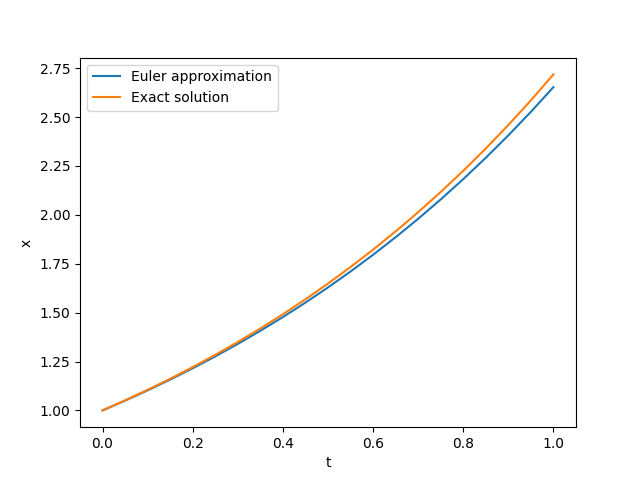
\includegraphics{linear_euler.png}
\cleardoublepage
        Finally, we show below that the numerical stability in Euler's method is
        lost when we increase again the time for which we try to approximate
        the solution.\\
        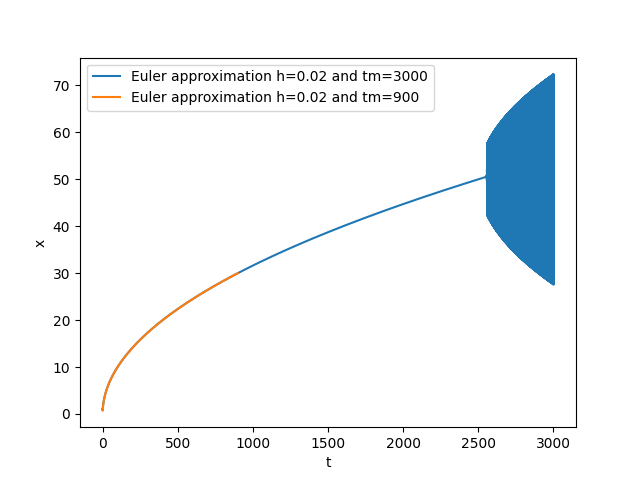
\includegraphics{nonlinear_euler.png}
	\end{proof}
\cleardoublepage
    \begin{proof}{\textbf{4.3}}
        Below is shown the functions used to calculate both the improved Euler's
        method and the Runge-Kutta method.
        \begin{verbatim}
            def imprvd_euler(x0, t0, h, tm=1):
                x, t = x0, t0
                while abs(t - tm) > (h / 2):
                    c1 = h * x
                    c2 = h * (x + c1)
                    x = x + 0.5 * (c1 + c2)
                    t = t + h
                print(f"h={h}, x(1)={x}, error={math.e - x}")


            def runge_kutta(x0, t0, h, tm=1):
                x, t = x0, t0
                while abs(t - tm) > (h / 2):
                    c1 = h * x
                    c2 = h * (x + (0.5 * c1))
                    c3 = h * (x + (0.5 * c2))
                    c4 = h * (x + c3)
                    x = x + 1/6 * (c1 + (2 * c2) + (2 * c3) + c4)
                    t = t + h
                print(f"h={h}, x(1)={x}, error={math.e - x}")
        \end{verbatim}
        And here is the output after looping through the different $h$ values
        \begin{verbatim}
            Improved Euler method
            h=0.1, x(1)=2.714080846608224, error=0.004200981850821073
            h=0.01, x(1)=2.7182368625599573, error=4.496589908775661e-05
            h=0.001, x(1)=2.7182813757517628, error=4.5270728232793545e-07

            Runge-Kutta method
            h=0.1, x(1)=2.718279744135166, error=2.0843238792700447e-06
            h=0.01, x(1)=2.7182818282344035, error=2.2464163862423447e-10
            h=0.001, x(1)=2.7182818284590247, error=2.042810365310288e-14
        \end{verbatim}
\cleardoublepage
    \end{proof}
    \begin{proof}{\textbf{4.4}}
        Let's compute one step of Runge-Kutta method for $f(x,t) = x$ with
        $x_0=1$ then
        \begin{align*}
            c_1 &= hx_0 = h\\
            c_2 &= h(x_0 + \frac{c_1}{2}) = h + \frac{h^2}{2} \\
            c_3 &= h(x_0 + \frac{c_2}{2}) = h + \frac{h^2}{2} + \frac{h^3}{4} \\
            c_4 &= h(x_0 + c_3) = h + h^2 + \frac{h^3}{2} + \frac{h^4}{4}\\
            x &= x_0 + \frac{(c_1 + 2c_2 + 2c_3 + c_4)}{6}
        \end{align*}
        By replacing the values of $x_0$, $c_1$, $c_2$, $c_3$ and $c_4$ we get that
        \begin{align*}
            x &= 1 + \frac{h + (2h + h^2) + (2h + h^2 + \frac{h^3}{2}) + (h + h^2 + \frac{h^3}{2} + \frac{h^4}{4})}{6} \\
              &= 1 + \frac{6h + 3h^2 + h^3 + \frac{h^4}{4}}{6} \\
              &= 1 + h + \frac{h^2}{2} + \frac{h^3}{6} + \frac{h^4}{24} \\
              &= 1 + h + \frac{h^2}{2!} + \frac{h^3}{3!} + \frac{h^4}{4!}
        \end{align*}
    \end{proof}
\cleardoublepage
    \begin{proof}{\textbf{4.6}}
        Expanding $x(t)$ as a taylor series we see that
        \begin{align*}
            x(t) = x(t_0) + (t - t_0)\dot{x}(t_0) +\frac{(t - t_0)^2}{2!}\ddot{x}(t_0)
        \end{align*}
        Let $h = t - t_0$ where $t_0 = 0$ then $x(h) = x(t-t_0) = x(t - 0) = x(t)$ then 
        \begin{align*}
            x(h) = x(0) + h\dot{x}(0) +\frac{h^2}{2!}\ddot{x}(0)      
        \end{align*}
        since $\dot{x} = f(x)$ then by the chain rule $\ddot{x}=f'(x)\dot{x}$
        and also we know that $x(0)=x_0$ so replacing we have that 
        \begin{align*}
            x(h) = x_0 + hf'(x_0) +\frac{h^2}{2!}f'(x_0)f(x_0)      
        \end{align*}
        Now let's compute one step of the \textit{Improved Euler method} when
        $x=x_0$ is the starting point
        \begin{align*}
            c_1 &= hf(x_0)\\
            c_2 &= hf(x_0+c_1)\\
            x &= x_0 + \frac{(c_1 + c_2)}{2}
        \end{align*}
        Expanding one term of the Taylor series of $f(x_0 + c_1)$ around $x_0$
        we get that 
        \begin{align*}
            f(x_0 + c_1) &= f(x_0) + ((x_0 + c_1) - x_0)f'(x_0)\\
                         &= f(x_0) + c_1f'(x_0)\\
                         &= f(x_0) + hf(x_0)f'(x_0)
        \end{align*}
        Then replacing $c_1$ and $c_2$ values using the taylor series expansion
        for $f(x_0 + c_1)$
        \begin{align*}
            x &= x_0 + \frac{hf(x_0)}{2} + \frac{h[f(x_0) + hf(x_0)f'(x_0)]}{2}\\
              &= x_0 + \frac{hf(x_0)}{2} + \frac{hf(x_0)}{2} + \frac{h^2f(x_0)f'(x_0)}{2}\\
              &= x_0 + hf(x_0) + \frac{h^2}{2}f(x_0)f'(x_0)
        \end{align*}

    \end{proof}
\end{document}























